\setcounter{page}{1}

\setcounter{section}{5}

\section{Introducción}

El presente documento reúne las actividades realizadas en el desarrollo de diversos proyectos relacionados con el Internet de las Cosas (IoT) y tecnologías asociadas, en el marco de un proyecto educativo desarrollado en la Universidad Autónoma Metropolitana Unidad Azcapotzalco.

El enfoque principal se centra en la integración de hardware y software para la monitorización, gestión y visualización de datos, aprovechando herramientas y tecnologías como microcontroladores (ESP8266 y ESP32), sensores, plataformas de desarrollo como Node-RED, bases de datos como InfluxDB y MySQL, y sistemas de visualización como Grafana.

Los resultados documentados en este trabajo representan una aproximación práctica al desarrollo de soluciones IoT, cubriendo desde la instalación y configuración de los entornos de desarrollo, hasta la implementación de sistemas completos de monitoreo en tiempo real.

\section{Objetivos generales y específicos}
    \subsection*{Objetivos generales}
    \begin{itemize}
        \item Diseñar e implementar un sistema de monitoreo basado en IOT que permite recopilar, procesar y visualizar datos en tiempo real.
        \item Facilitar la replicación y escalabilidad del proyecto mediante una documentación técnica detallada y el uso de Docker como herramienta de contenedorización.
    \end{itemize}
    \subsection*{Objetivos específicos}
    \begin{itemize}
        \item Configurar el entorno de desarrollo para trabajar con microcontroladores ESP32 y ESP8266.
        \item Implementar proyectos individuales con sensores conectados a un microcontrolador para preparar la integración con el sistema de monitoreo.
        \item Desplegar los servicios de InfluxDB, MySQL, Node-RED y Grafana en contenedores Docker sobre una Raspberry Pi.
        \item Diseñar flujos en Node-RED para integrar los datos recopilados y enviar alertas personalizadas por Telegram en caso de detectar anomalías.
        \item Crear dashboards en Grafana para visualizar datos históricos y en tiempo real provenientes de los sensores IoT.
        \item Documentar cada paso del proceso de desarrollo, desde la configuración inicial del entorno hasta la implementación y visualización final, con el fin de garantizar la reproducibilidad del proyecto.
    \end{itemize}

\section{Metología utilizada}

La metodología empleada para el desarrollo de este proyecto se diseñó con base en un enfoque modular, asegurando que cada componente, desde la configuración de software hasta la implementación de hardware, fuera integrado de manera eficiente y documentado en detalle. A continuación, se describen los pasos principales:

\begin{itemize}
    \item \textbf{Preparación del entorno de desarrollo:} Configuración de Linux Mint como sistema operativo base y la instalación de herramientas como Visual Studio Code, Arduino IDE y MQTTX.
    \item \textbf{Configuración de la Raspberry Pi como servidor IoT:} Instalación de Raspberry Pi OS, Docker y despliegue de servicios como EMQX, InfluxDB, MySQL, Node-RED y Grafana.
    \item \textbf{Desarrollo de proyectos individuales:} Implementación de proyectos con microcontroladores ESP32 y ESP8266, integrando sensores de temperatura, humedad, luz y gas.
    \item \textbf{Comunicación y almacenamiento de datos:} Establecimiento de comunicación entre los sensores y el servidor mediante MQTT, creación de flujos en Node-RED para procesar y enviar datos a las bases de datos, y generación de alertas por Telegram.
    \item \textbf{Visualización de datos en Grafana:} Creación de dashboards personalizados para visualizar datos en tiempo real y de forma histórica.
    \item \textbf{Documentación del proyecto:} Creación de una página web con tutoriales, guías y ejemplos de código para facilitar la comprensión y replicabilidad del proyecto.
\end{itemize}

\section{Actividades realizadas}

A continuación, se detallan las actividades realizadas durante el desarrollo del proyecto, abarcando desde la preparación del entorno de desarrollo hasta la implementación y visualización de los datos recopilados.

\subsection*{Configuración del entorno de desarrollo}

\begin{itemize}
    \item \textbf{Instalación de Linux Mint:} Se configuró como sistema operativo base para desarrollar el proyecto, asegurando compatibilidad con las herramientas requeridas.
    \item \textbf{Instalación de herramientaa:}
    \begin{itemize}
        \item \textbf{Visual Studio Code:} con la extensión PlatformIO para programar los microcontroladores ESP32 y ESP8266.
        \item \textbf{Arduino IDE:} como alternativa para utilizar el serial protter y graficar datos de los sensores.
        \item \textbf{MQTTX:} para probar la comunicación MQTT entre los dispositivos y el broker.
    \end{itemize}
\end{itemize}

\subsection*{Configuración de la Raspberry Pi como servidor IoT}

\begin{itemize}
    \item \textbf{Instalación de Raspberry Pi OS:} Configuración del sistema operativo en la Raspberry Pi y la habilitación de SSH para acceder de forma remota.
    \item \textbf{Instalación de Docker:} Instalación y configuración para desplegar los servicios en contenedores de manera automática al iniciar la Raspberry Pi.
    \item \textbf{Despliegue y configuración de servicios:}
    \begin{itemize}
        \item \textbf{EMQX:} como broker MQTT para la comunicación entre los sensores y el servidor.
        \item \textbf{InfluxDB:} para almacenar datos de series temporales provenientes de los sensores.
        \item \textbf{MySQL:} para el almacenamiento de los usuarios a los que se enviarán las alertas.
        \item \textbf{Node-RED:} para la creación de flujos de datos y la integración con los servicios anteriores.
        \item \textbf{Grafana:} para la visualización de los datos en dashboards personalizados.
    \end{itemize}
\end{itemize}

\subsection*{Desarrollo de proyectos individuales}

\begin{itemize}
    \item \textbf{Microcontroladores ESP8266 y ESP32:} Configuración de pines, conexión a redes Wi-Fi y ejecución de pruebas básicas.
    \item \textbf{Integración de sensores:} \begin{itemize}
        \item \textbf{DHT:} para medir temperatura y humedad.
        \item \textbf{BH1750:} para medir la intensidad de la luz.
        \item \textbf{MQ:} para detectar la presencia de gas. 
    \end{itemize}
    \item \textbf{Implementación de una pantalla LCD 16x2:} Configuración con interfaz I2C para mostrar lecturas en tiempo real de los sensores.
\end{itemize}

\subsection*{Comunicación y almacenamiento de datos}

\begin{itemize}
    \item \textbf{Flow para enviar alertas:} Creación de un flujo en Node-RED para enviar alertas por Telegram de forma automática y personalizada en caso de detectar anomalías.
    \item \textbf{Flow para guardar datos en InfluxDB:} Configurar un flujo para almacenar en influxDB los datos de los sensores enviados a través de MQTT.
    \item \textbf{Flow para almacenar usuarios en MySQL:} Creación de un flujo para almacenar los usuarios a los que se enviarán las alertas en una base de datos MySQL desde Telegram.
    \item \textbf{Creación de dashboards en Grafana:} Diseño de dashboards personalizados para visualizar los datos de los sensores en tiempo real y de forma histórica.
\end{itemize}

\subsection*{Documentación del proyecto}

Se documentó cada paso del proceso de desarrollo en una página web, incluyendo tutoriales de instalación, guías de configuración y ejemplos de código. Esto asegura la replicabilidad del proyecto y facilita la comprensión de los conceptos y tecnologías utilizadas.

\section{Objetivos y metas alcanzadas}

\begin{itemize}
    \item Configuración del entorno de desarrollo para trabajar con los microcontroladores ESP32 y ESP8266.
    \item Implementación de proyectos individuales con sensores como el de temperatura, humedad, luz y gas a un microcontrolador para la integración con el sistema de monitoreo.
    \item Despliegue de servicios de InfluxDB, MySQL, Node-RED y Grafana en contenedores Docker sobre una Raspberry Pi para la gestión y visualización de datos.
    \item Establecimiento de comunicación entre los sensores y el servidor mediante el protocolo MQTT.
    \item Creación de flujos en Node-RED para procesar y enviar datos a las bases de datos y generar alertas mediante Telegram.
    \item Creación de dashboards en Grafana para visualizar datos históricos y en tiempo real provenientes de los sensores IoT.
    \item Documentación detallada que abarca desde la configuración de herramientas hasta la implementación y el despliegue del proyecto en una página web, diseñada para ser fácil de usar y comprender.
\end{itemize}

\section{Resultados y conclusiones}

\subsection*{Circuito del proyecto}

El circuito completo después de juntar todos los proyectos individuales se muestra en la figura~\ref{fig:proyectos}. En la figura~\ref{fig:esp8266} se muestra el circuito con los sensores conectados a un ESP8266 y en la figura~\ref{fig:esp32} se muestra el circuito con los sensores conectados a un ESP32.

\begin{figure}[H]
    \centering
    \begin{subfigure}[b]{0.45\linewidth}
        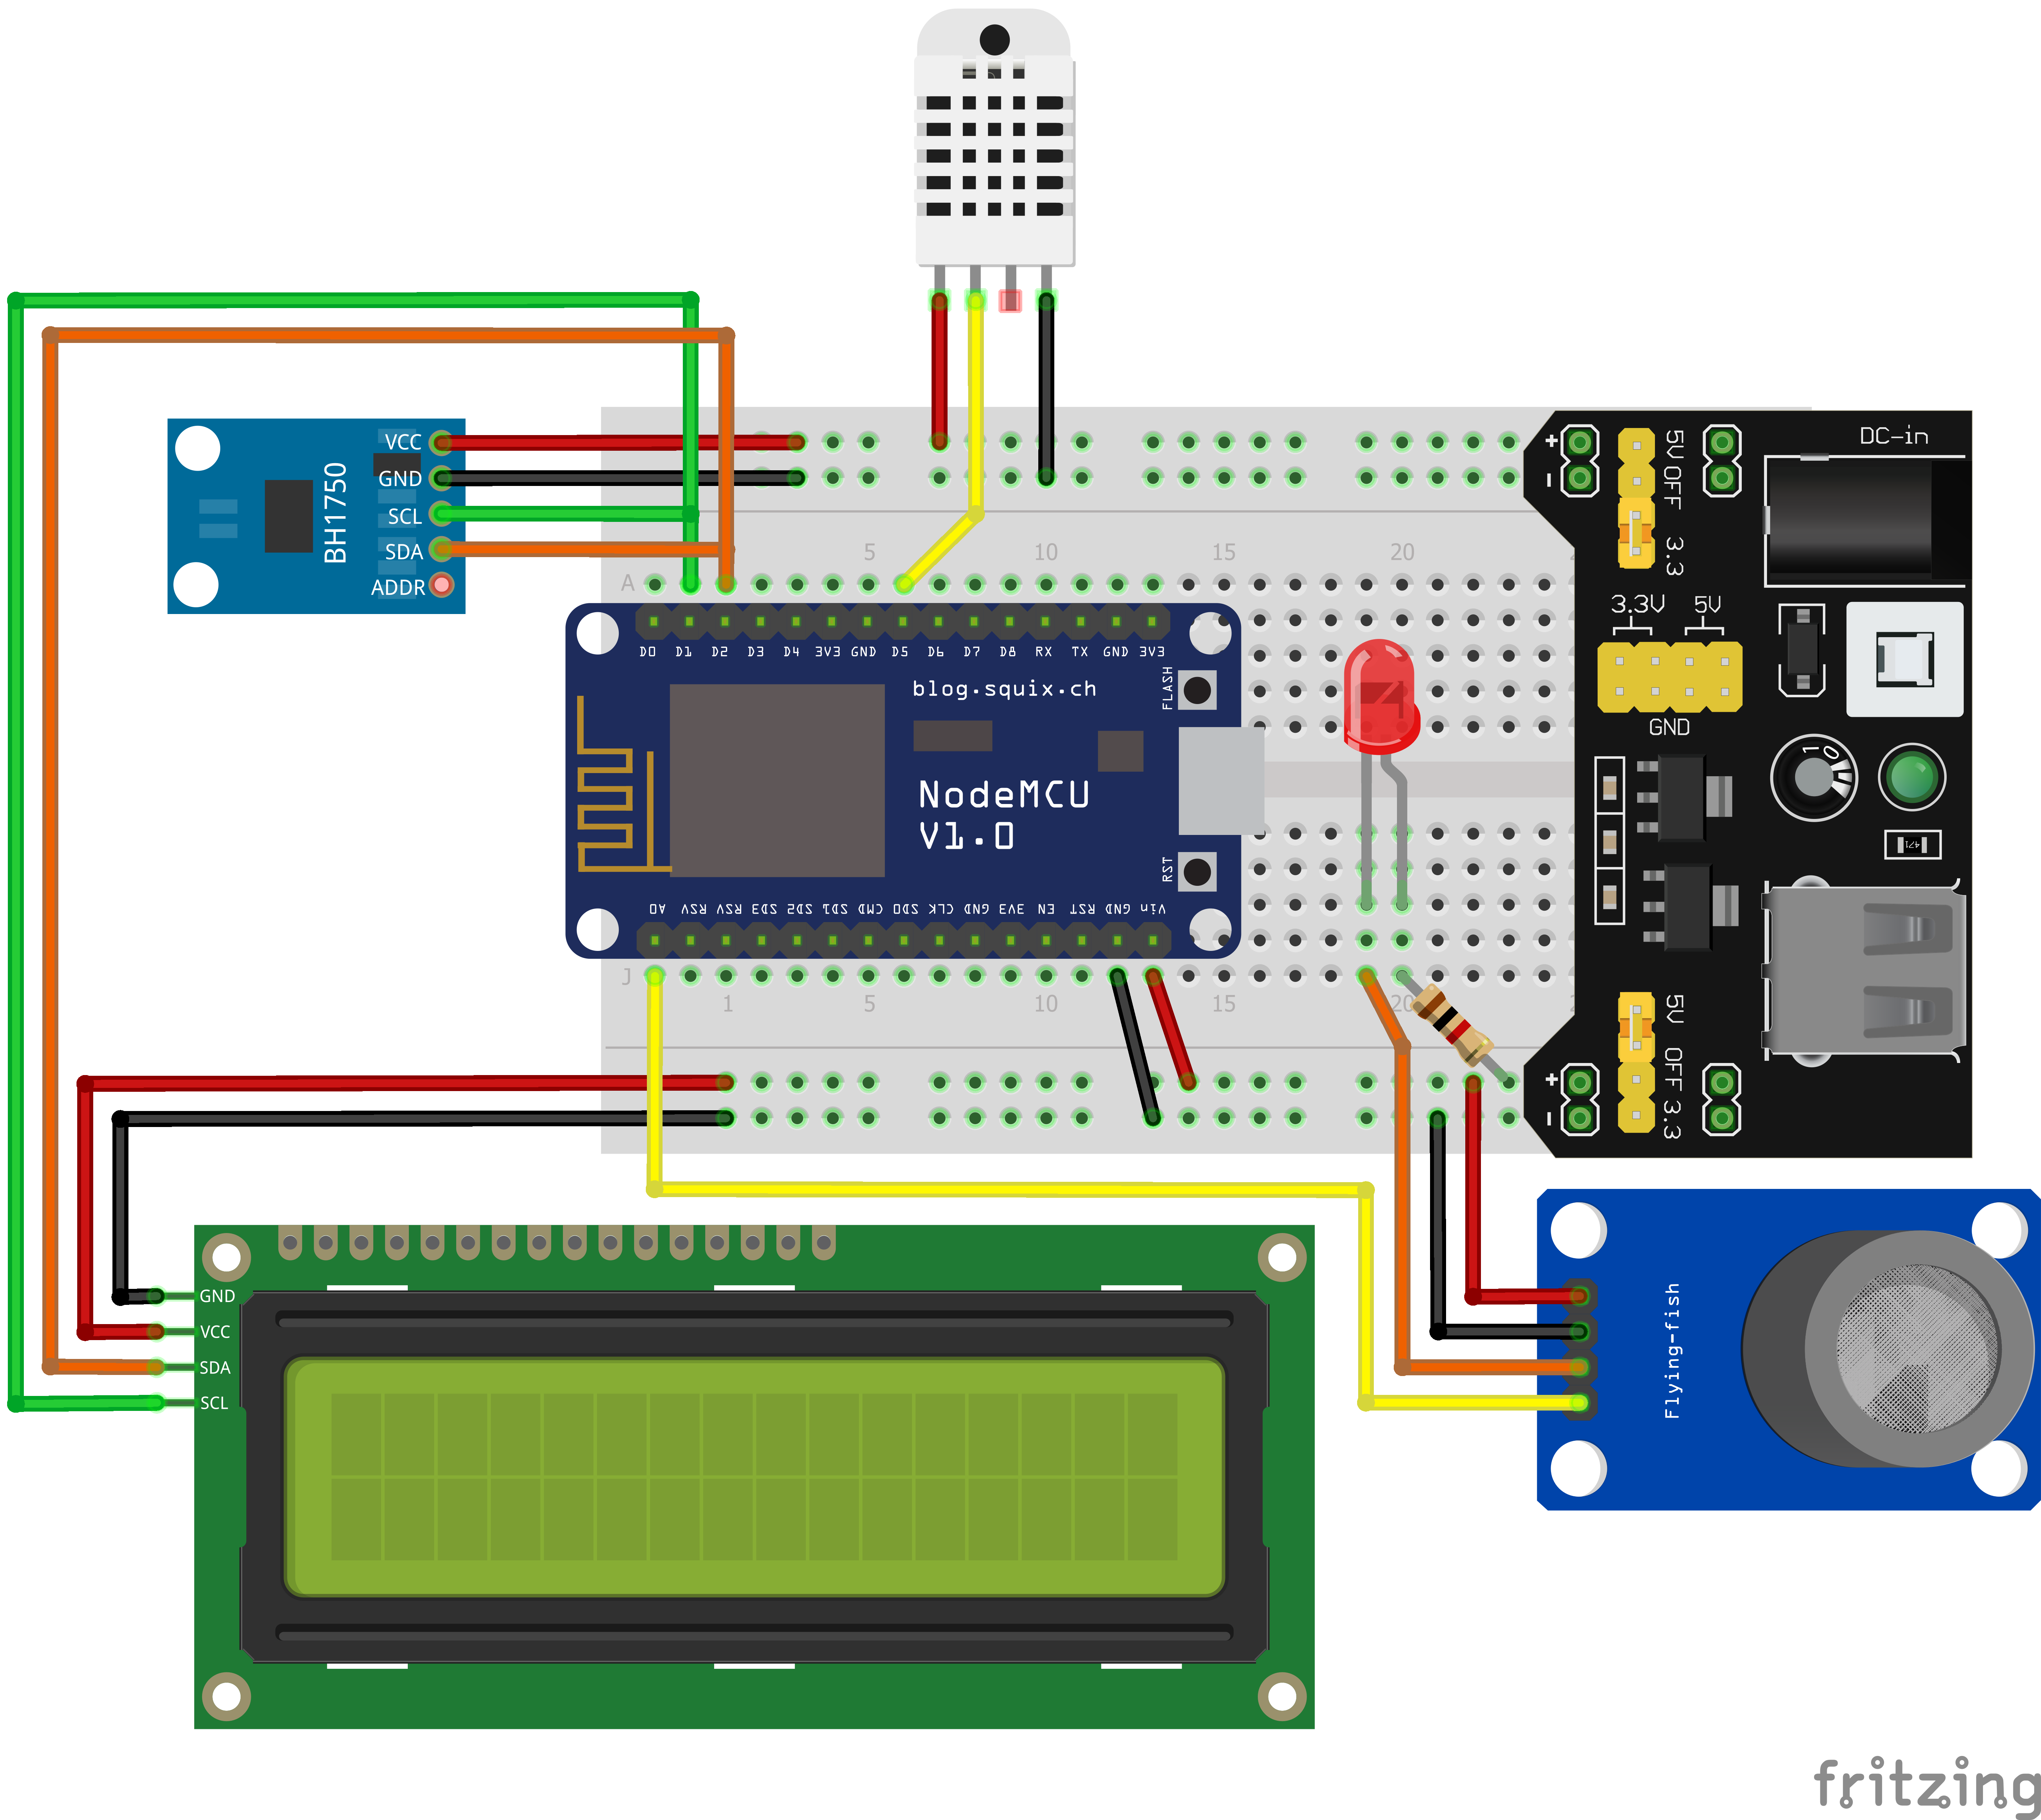
\includegraphics[width=\linewidth]{img/proyecto_esp8266.png}
        \caption{Sensores conectados a un ESP8266}
        \label{fig:esp8266}
    \end{subfigure}
    \begin{subfigure}[b]{0.45\linewidth}
        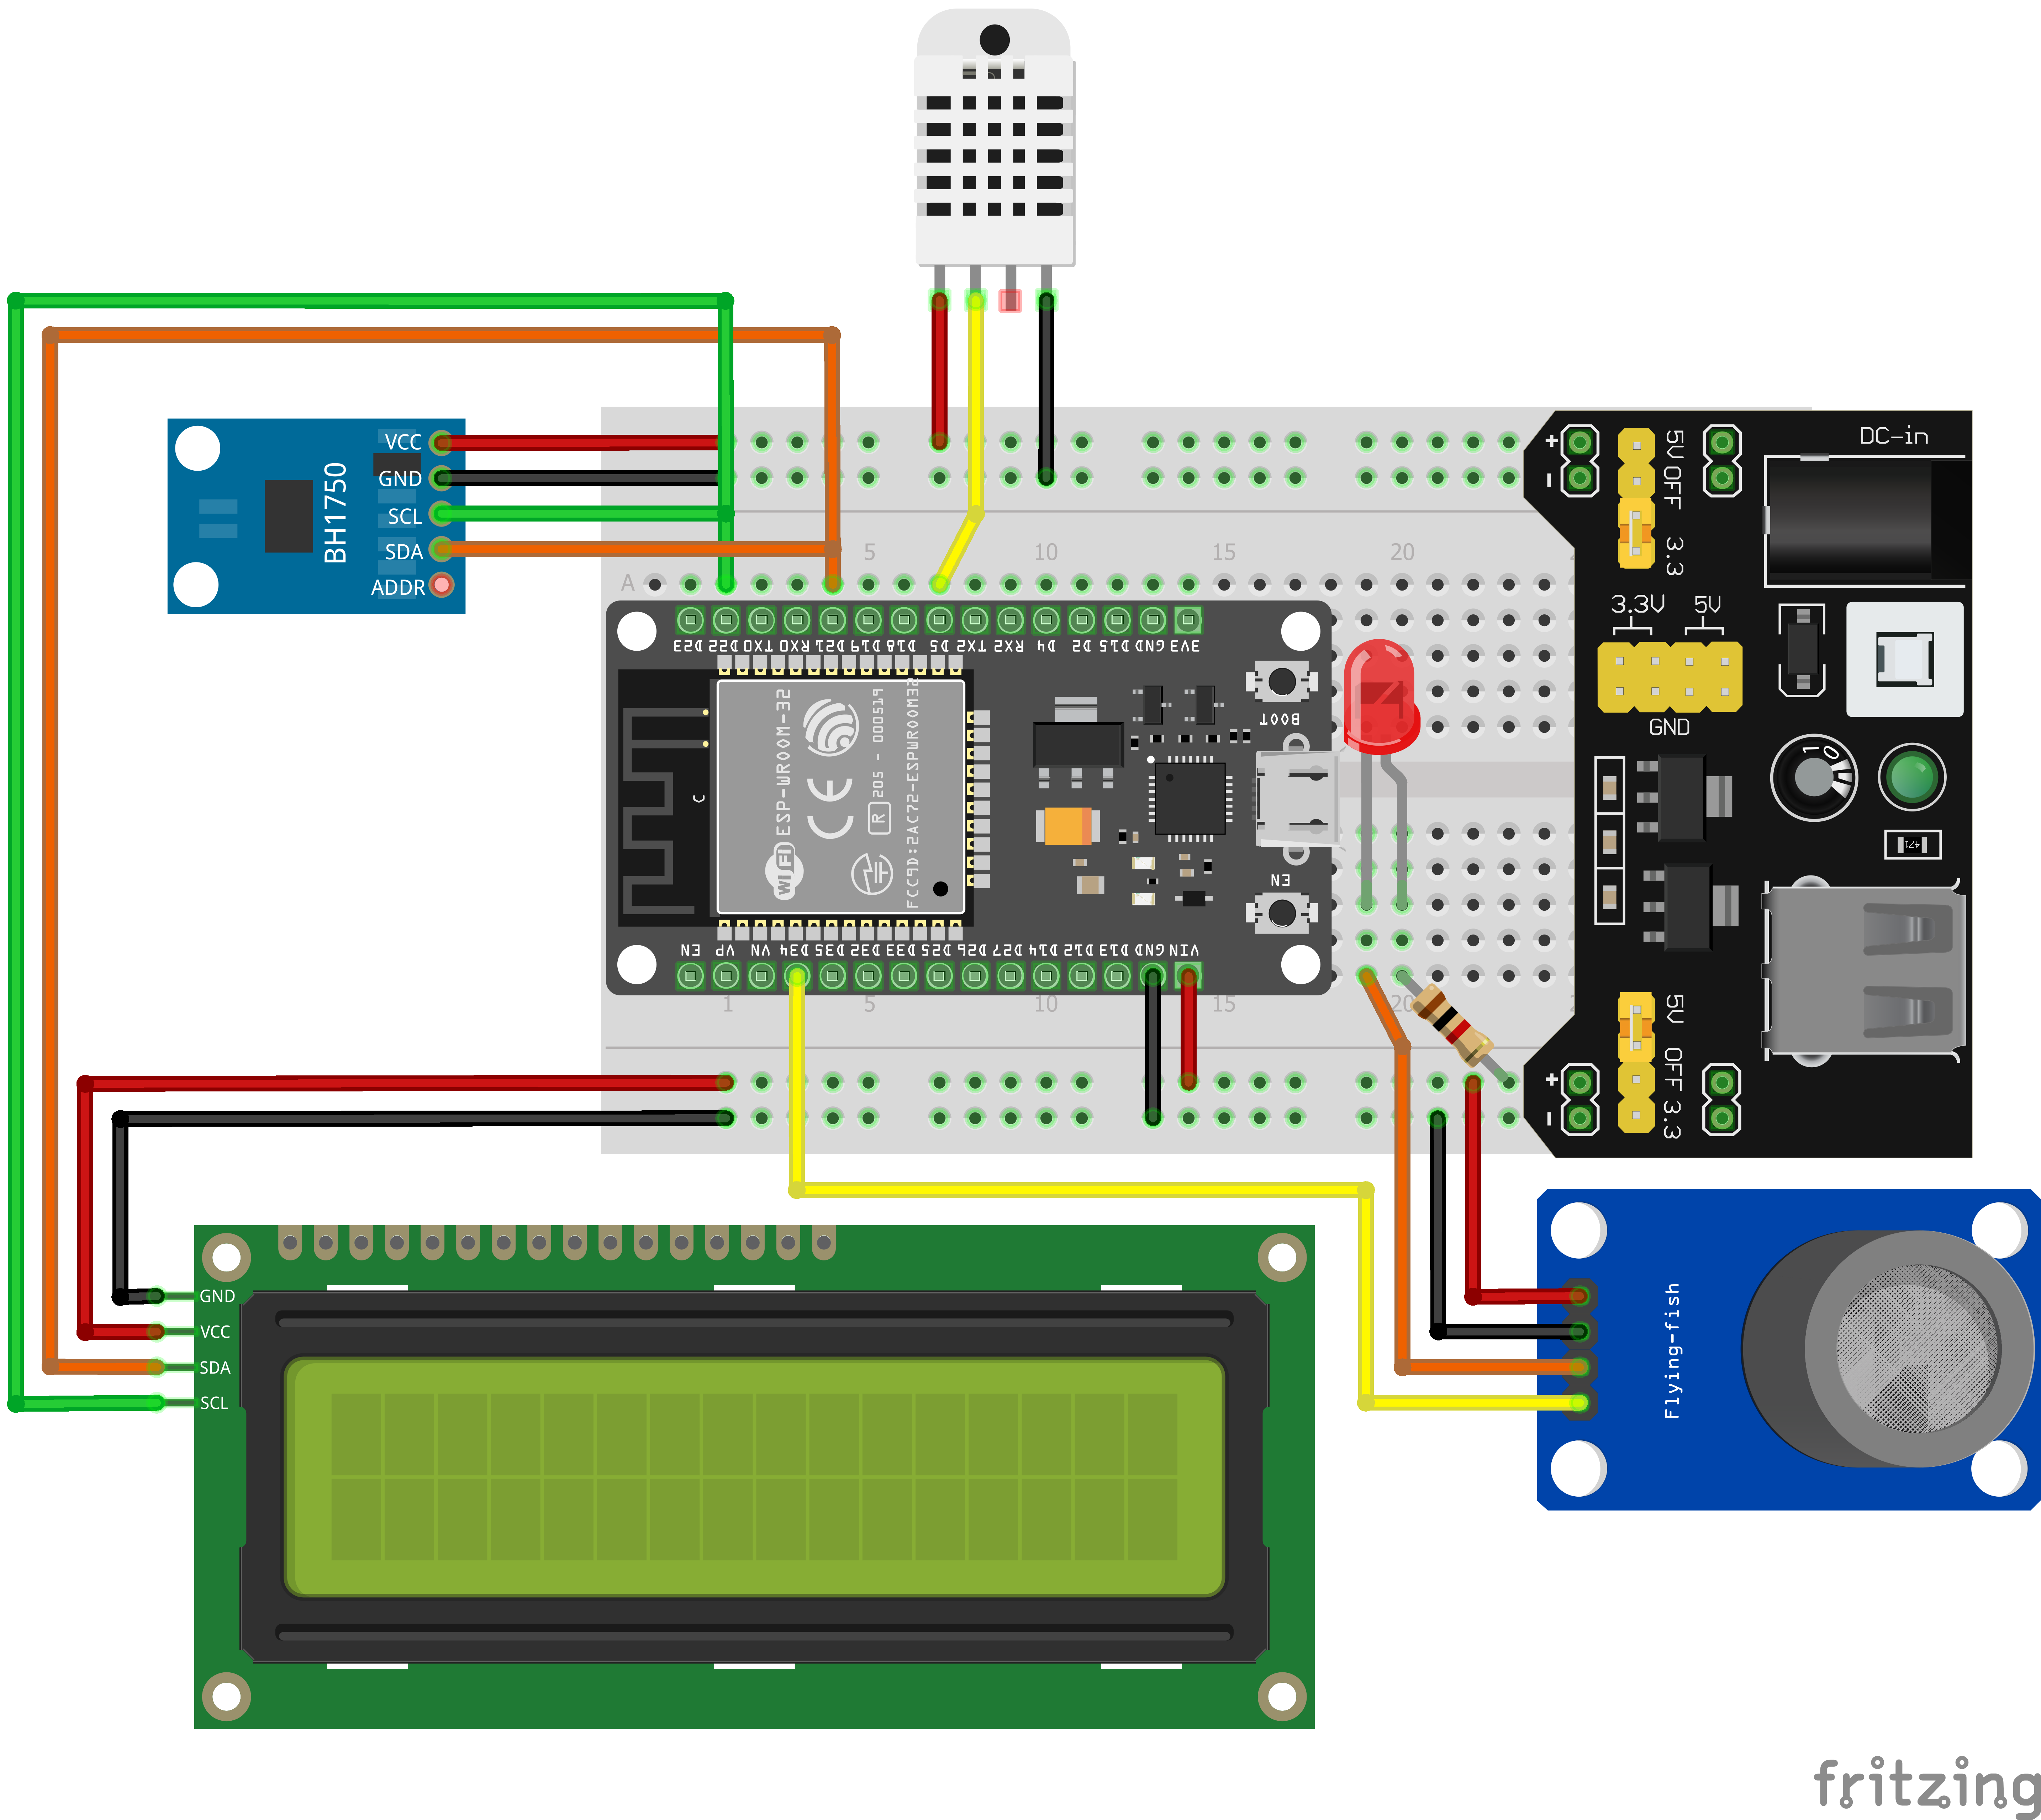
\includegraphics[width=\linewidth]{img/proyecto_esp32.png}
        \caption{Sensores conectados a un ESP32}
        \label{fig:esp32}
    \end{subfigure}
    \caption{Circuitos del proyecto}
    \label{fig:proyectos}
\end{figure}

Para enviar los datos de los sensores al servidor, primero es necesario conectarse a Internet. Para simplificar este proceso, al encender el microcontrolador, este creará un hotspot al que podremos conectarnos para configurar las credenciales de la red a la que se conectará. En la figura~\ref{fig:credenciales} se muestra la página web que se despliega al conectarse al hotspot del microcontrolador. Una vez ingresadas las credenciales de la red, el microcontrolador se conectará a Internet y enviará los datos por MQTT al servidor.

\begin{figure}[H]
    \centering
    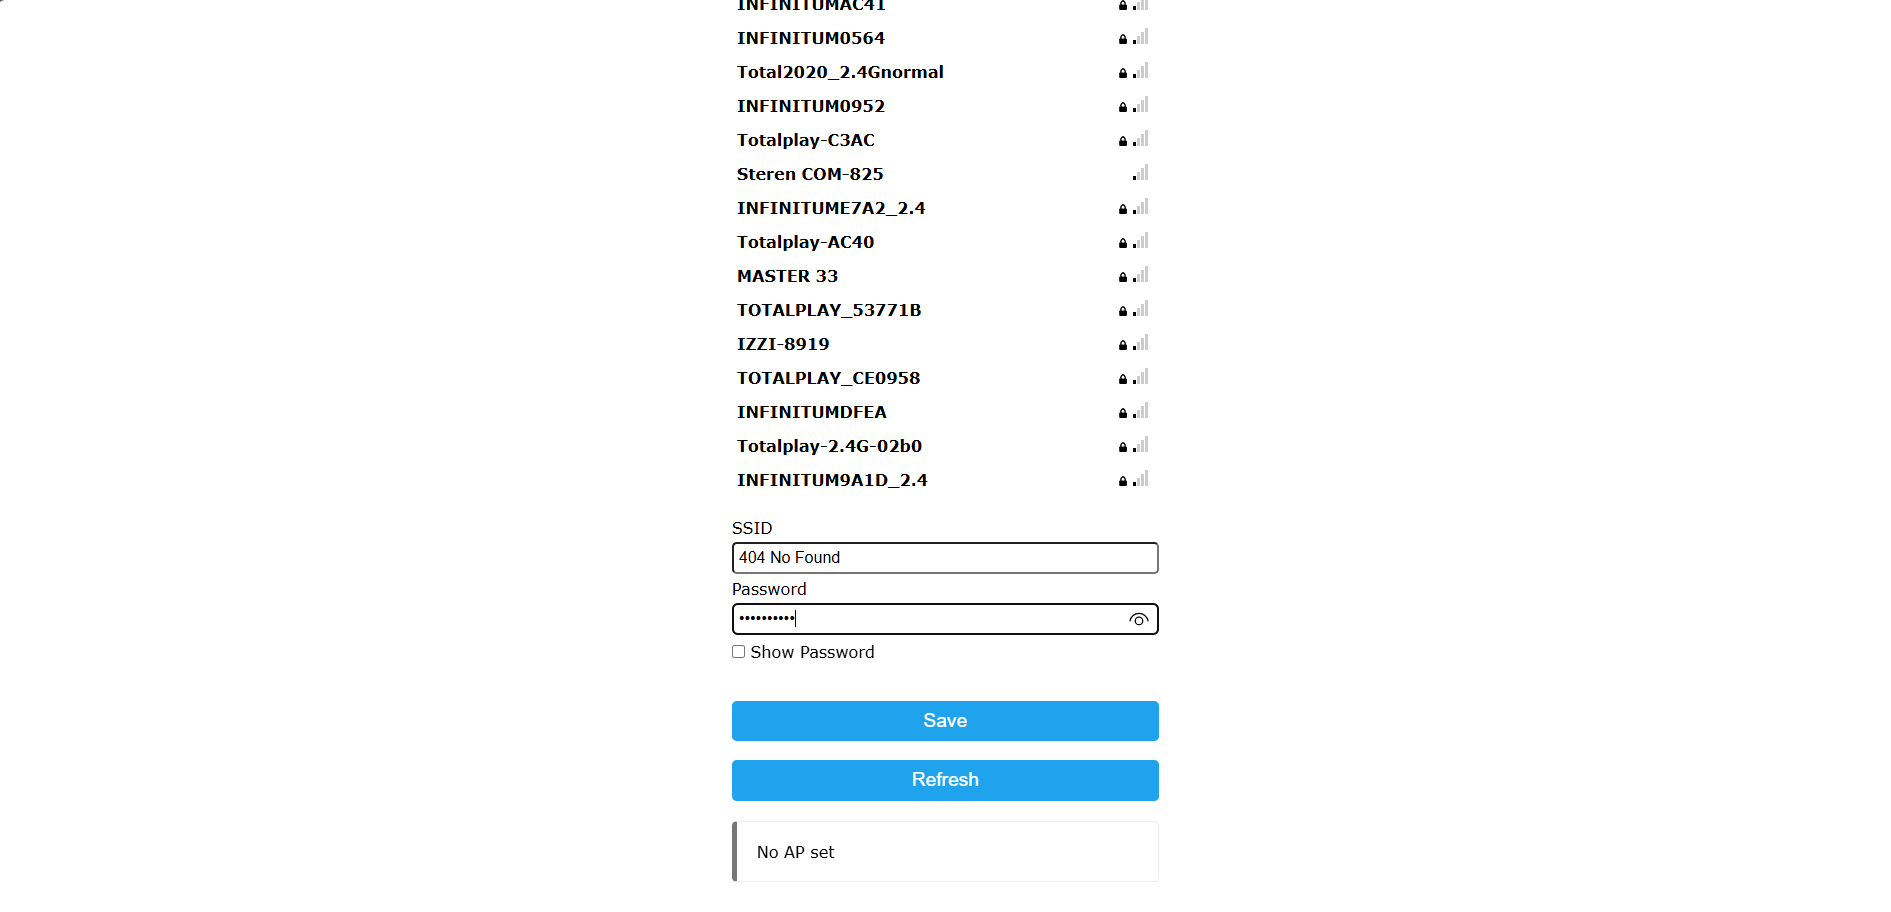
\includegraphics[width=0.8\textwidth]{img/proyecto_credenciales.png}
    \caption{Página web para configurar las credenciales de la red}
    \label{fig:credenciales}
\end{figure}


\subsection*{Guardar información de los sensores y enviar alertas personalizadas}

Los datos enviados por los sensores se almacenan en una base de datos InfluxDB. En la figura~\ref{fig:influxdb} se puede ver el flujo de Node-RED que se encarga de guardar los datos en la base de datos después de recibirlos por MQTT.

\begin{figure}[H]
    \centering
    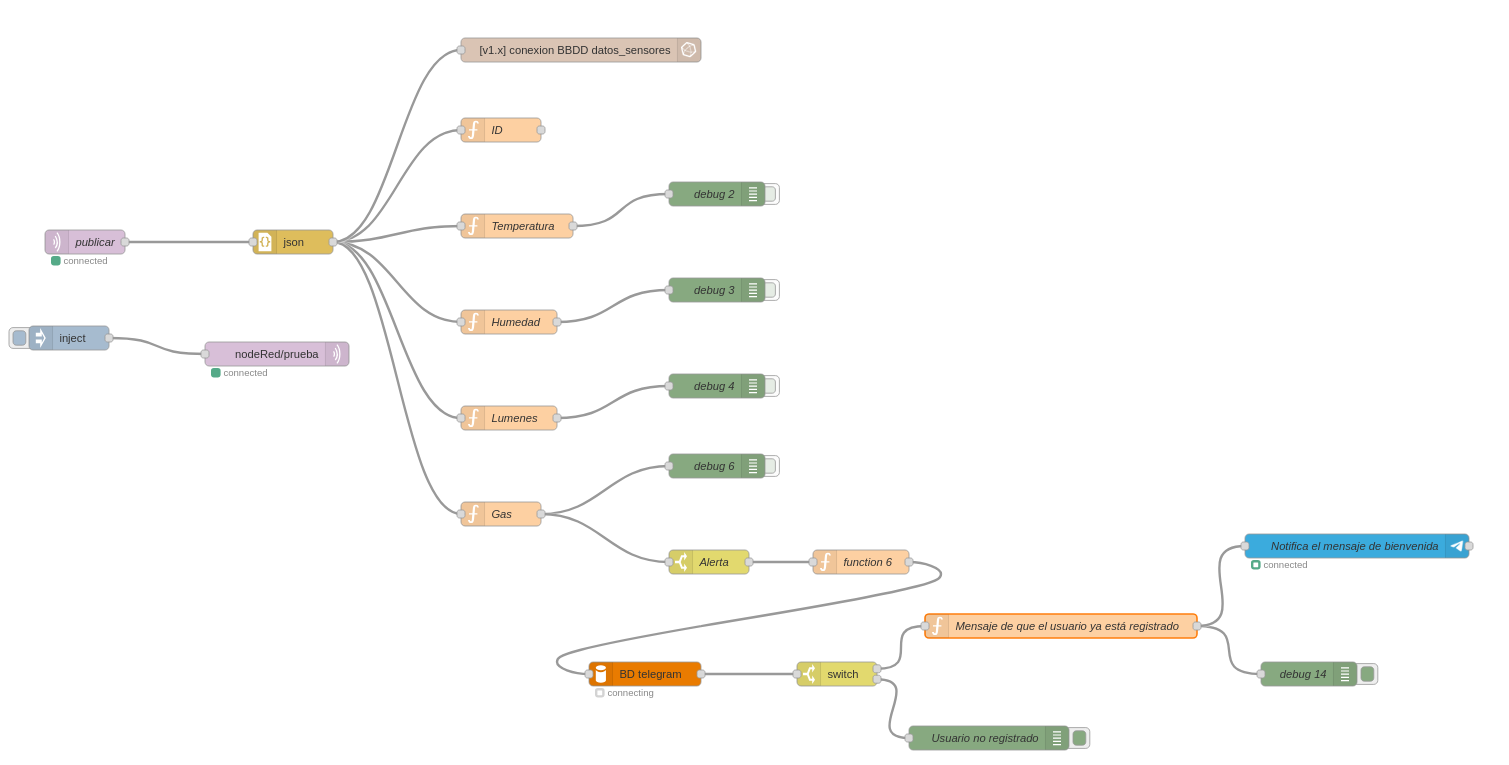
\includegraphics[width=0.8\textwidth]{img/flow_baseDatos.png}
    \caption{Flujo de Node-RED para guardar datos en InfluxDB}
    \label{fig:influxdb}
\end{figure}

El flujo anterior también se encarga de enviar alertas personalizadas a través de Telegram cuando se detectan anomalías en los datos recibidos por MQTT. En la figura~\ref{fig:telegram} se muestra un mensaje de alerta personalizado enviado por Telegram, el cual se envía únicamente a los usuarios registrados.

\begin{figure}[H]
    \centering
    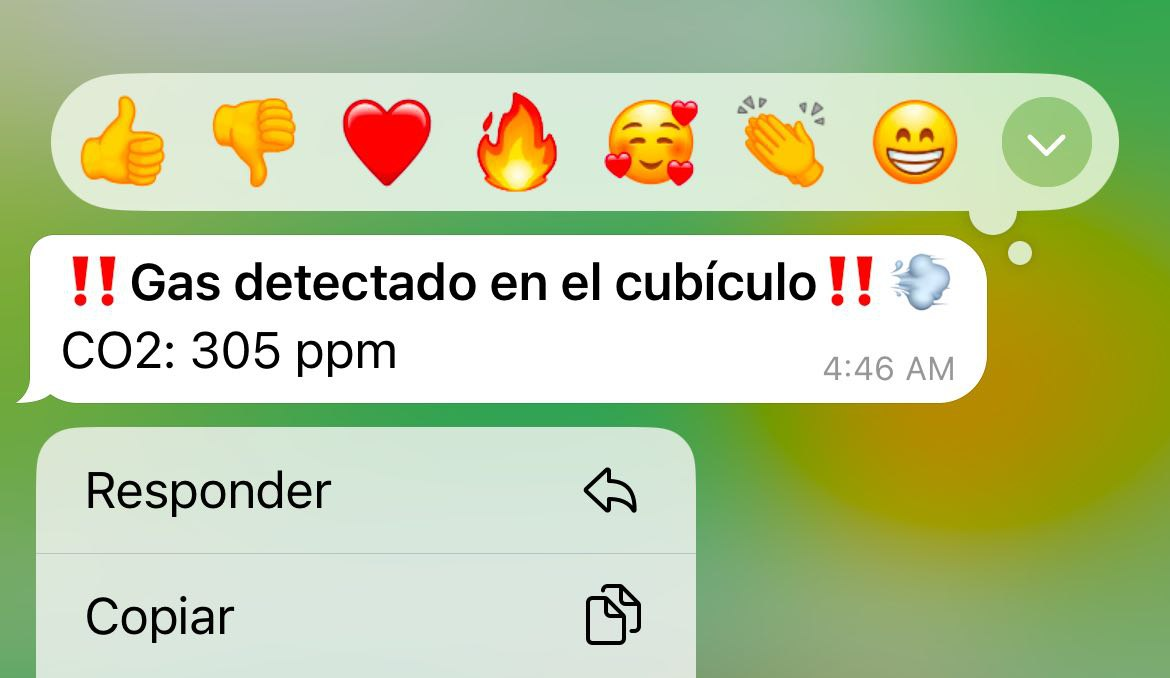
\includegraphics[width=0.6\textwidth]{img/telegram_alerta.jpg}
    \caption{Alerta enviada por telegram}
    \label{fig:telegram}
\end{figure}

\subsection*{Registrar un usuario para recibir alertas}

Para registrar un usuario y recibir alertas personalizadas por Telegram, es necesario enviar un mensaje al bot de Telegram con el comando \texttt{/start}. En la figura~\ref{fig:registro} se muestra el flujo de Node-RED que se encarga de registrar a los usuarios en una base de datos MySQL.

\begin{figure}[H]
    \centering
    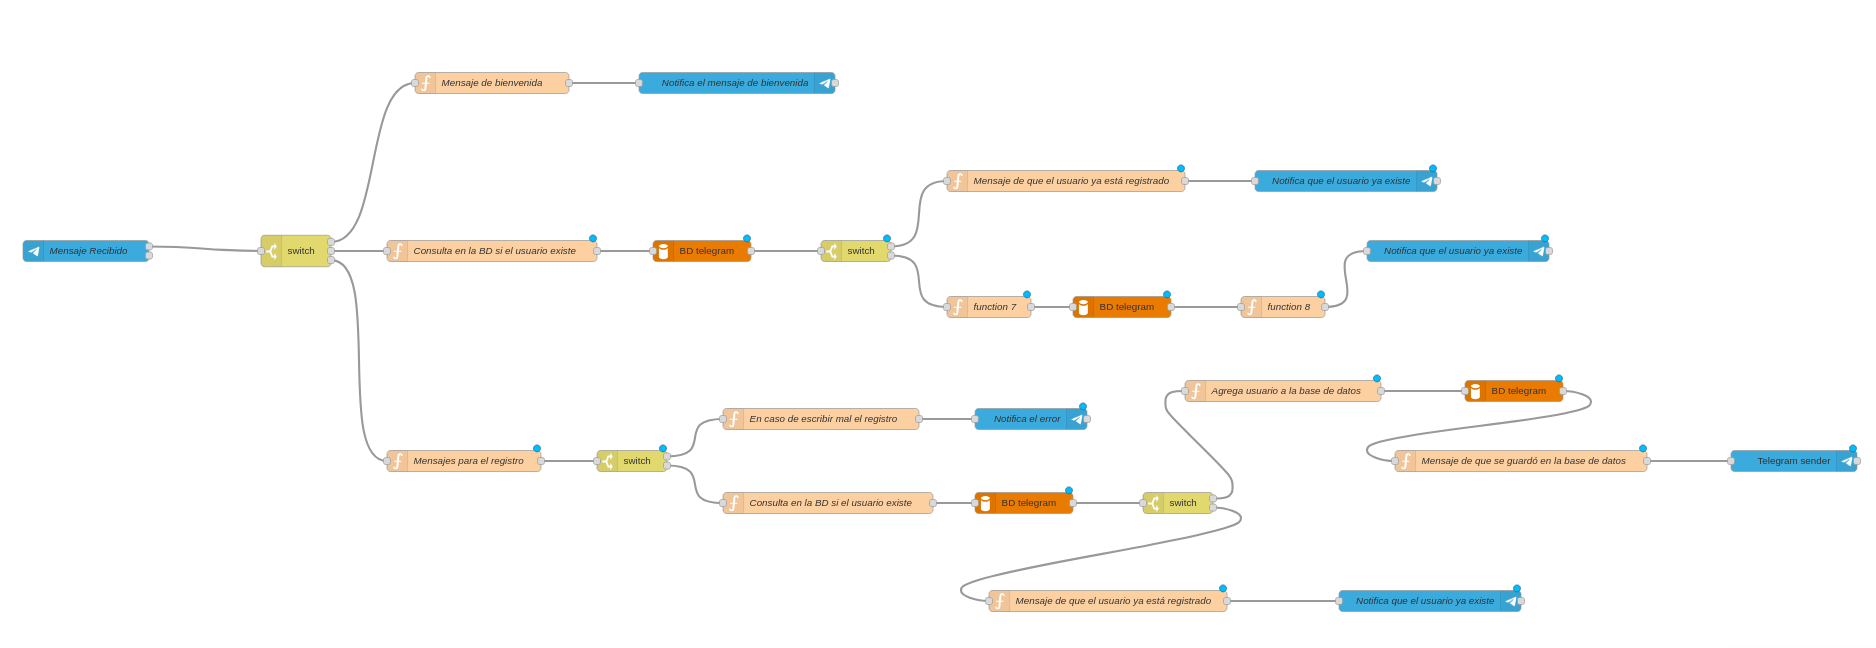
\includegraphics[width=0.8\textwidth]{img/flow_telegram.png}
    \caption{Flujo de Node-RED para registrar usuarios en MySQL}
    \label{fig:registro}
\end{figure}

El flujo anterior se activa cuando un usuario envía el comando \texttt{/start} al bot de Telegram. En la figura~\ref{fig:registro_telegram} se muestra la interacción con el bot de Telegram para registrar un usuario.

\begin{figure}[H]
    \centering
    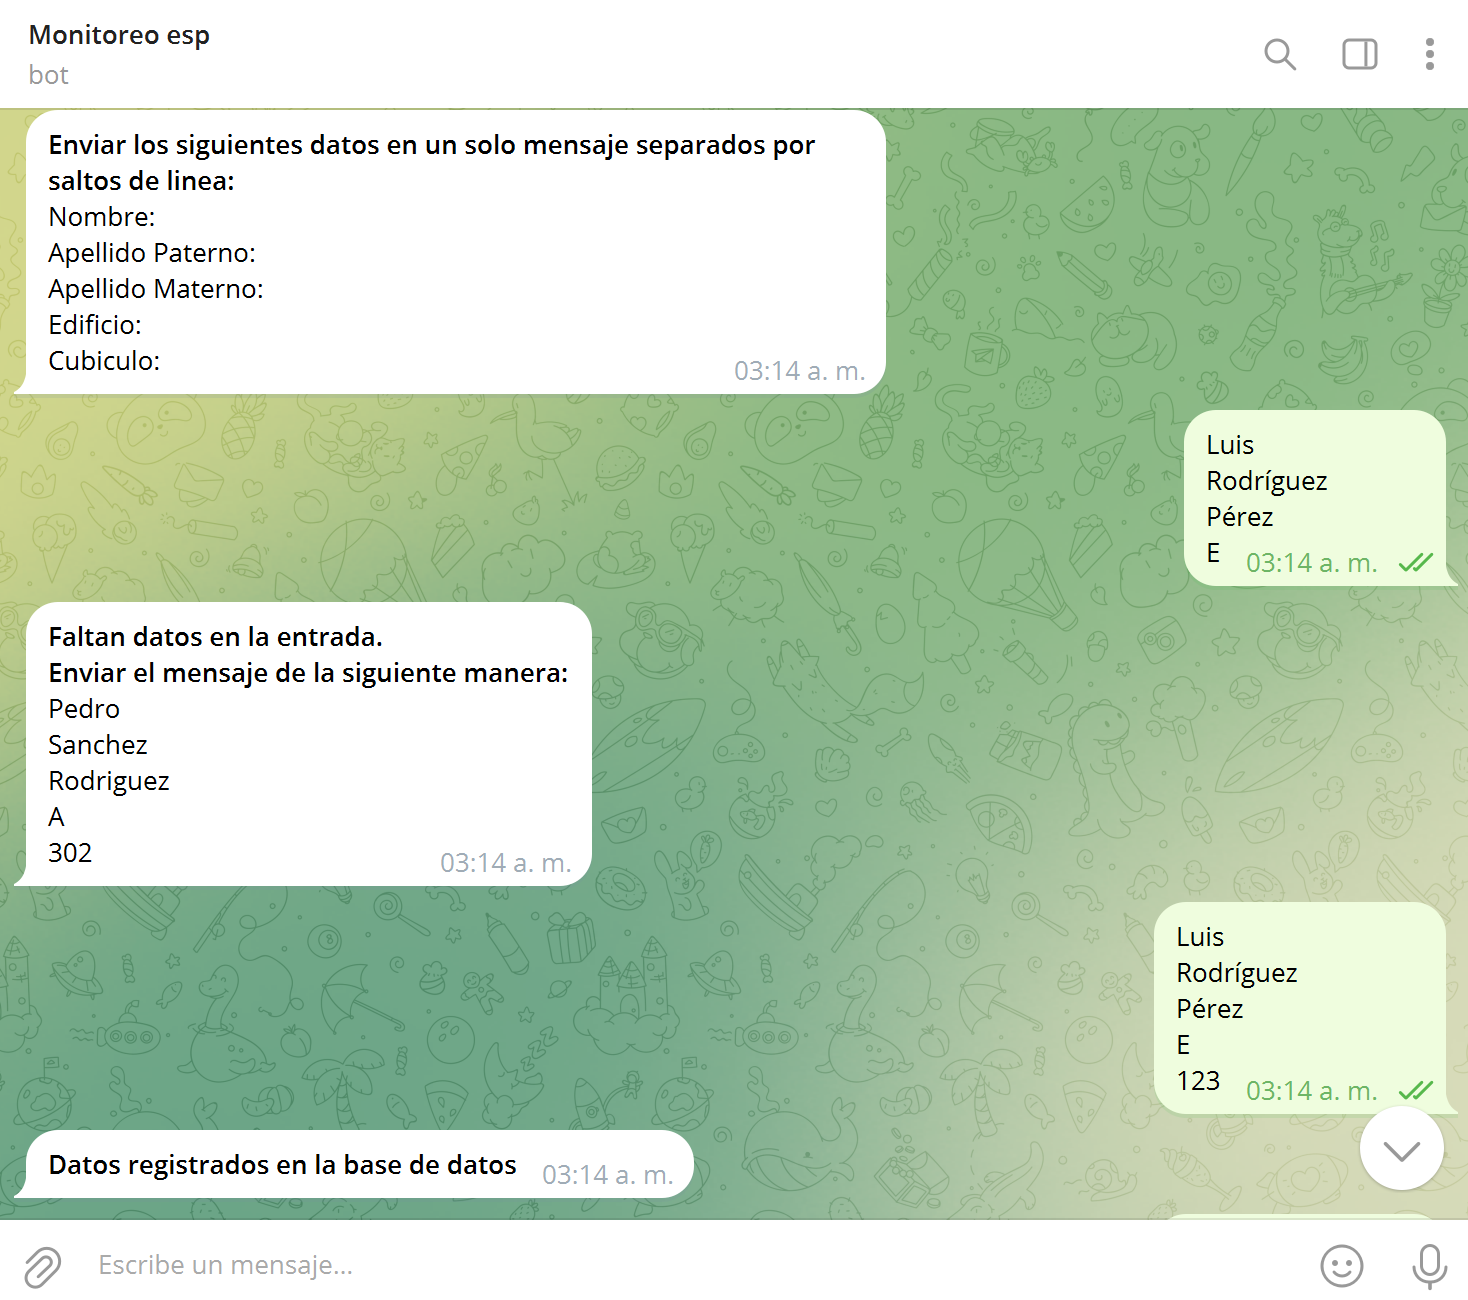
\includegraphics[width=0.6\textwidth]{img/proyecto_telegram.png}
    \caption{Registro de un usuario en Telegram}
    \label{fig:registro_telegram}
\end{figure}

\subsection*{Visualización de datos en Grafana}

Los datos almacenados en InfluxDB se visualizan en dashboards personalizados en Grafana. Estos datos son tomados desde la base de datos InfluxDB y se actualizan en tiempo real. En la figura~\ref{fig:grafana} se muestra un dashboard con los datos de temperatura, humedad, luz y gas en tiempo real.

\begin{figure}[H]
    \centering
    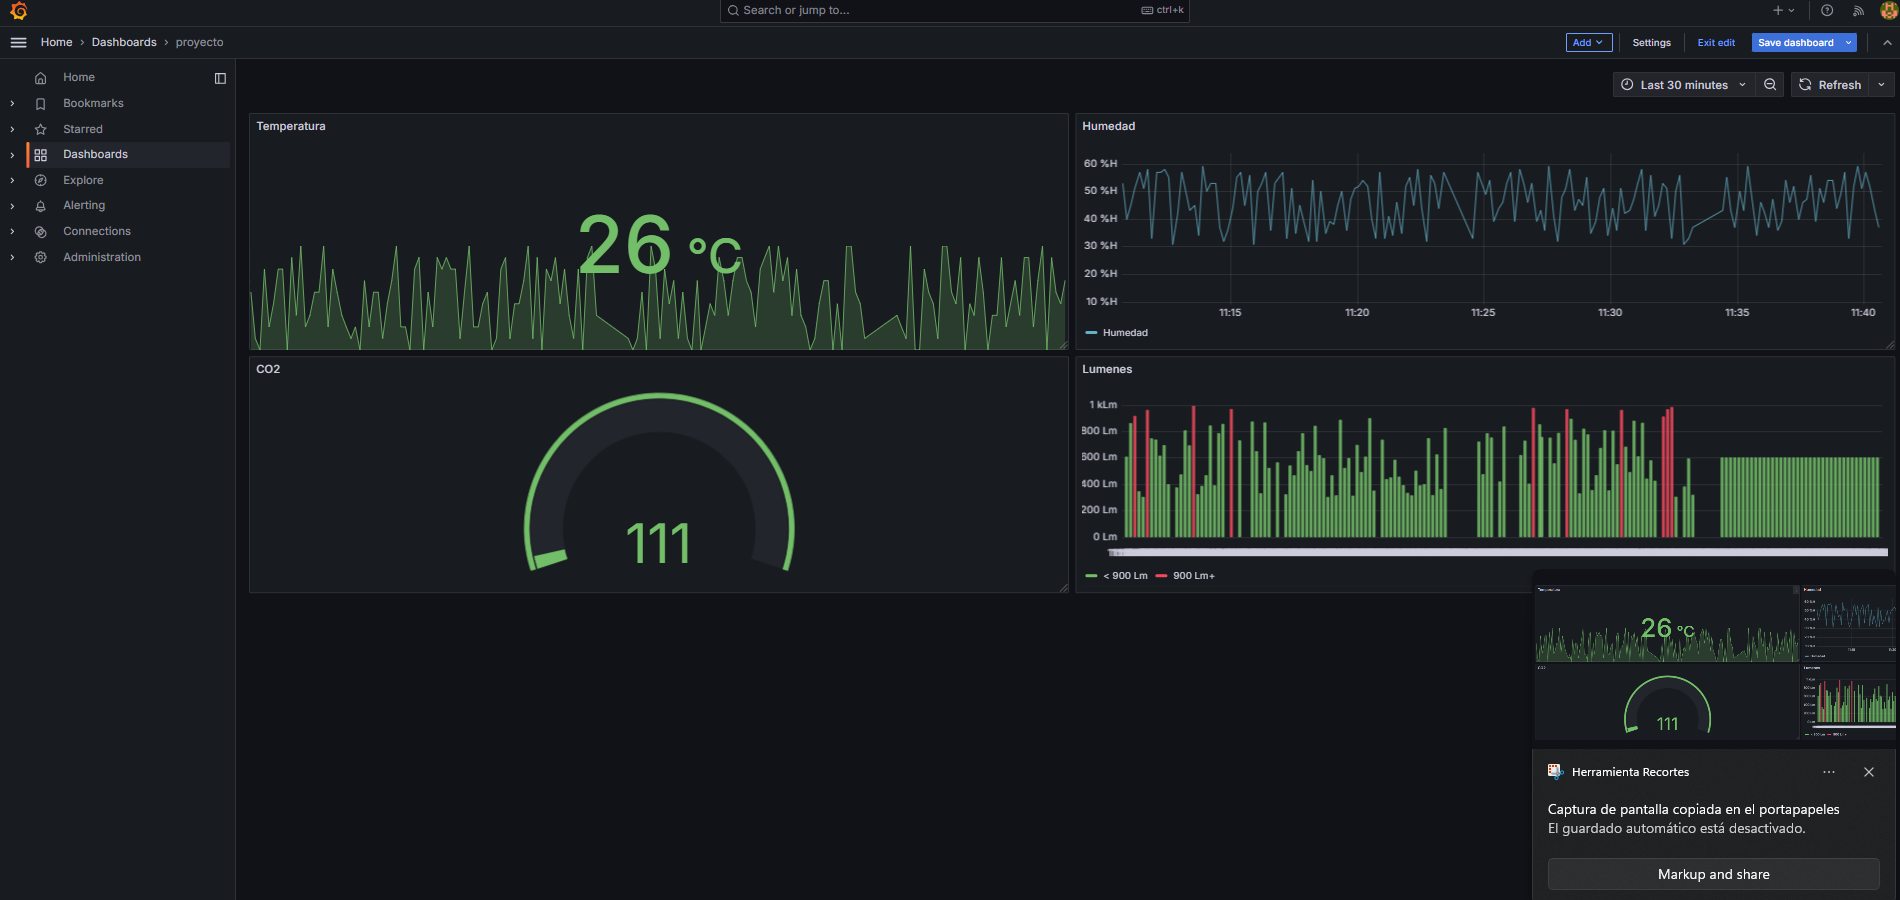
\includegraphics[width=0.8\textwidth]{img/proyecto_grafana.png}
    \caption{Dashboard en Grafana con los datos de los sensores}
    \label{fig:grafana}
\end{figure}

\subsection*{Documentación del proyecto}

La documentación del proyecto fue publicada en github pages y se puede acceder a través del siguiente enlace: \url{https://luisangel2801.github.io/Servicio-Social/}. Este sitio web contiene tutoriales, guías y ejemplos de código para facilitar la comprensión y replicabilidad del proyecto. En la figura~\ref{fig:paginaWeb} se muestra la página principal de la documentación.

\begin{figure}[H]
    \centering
    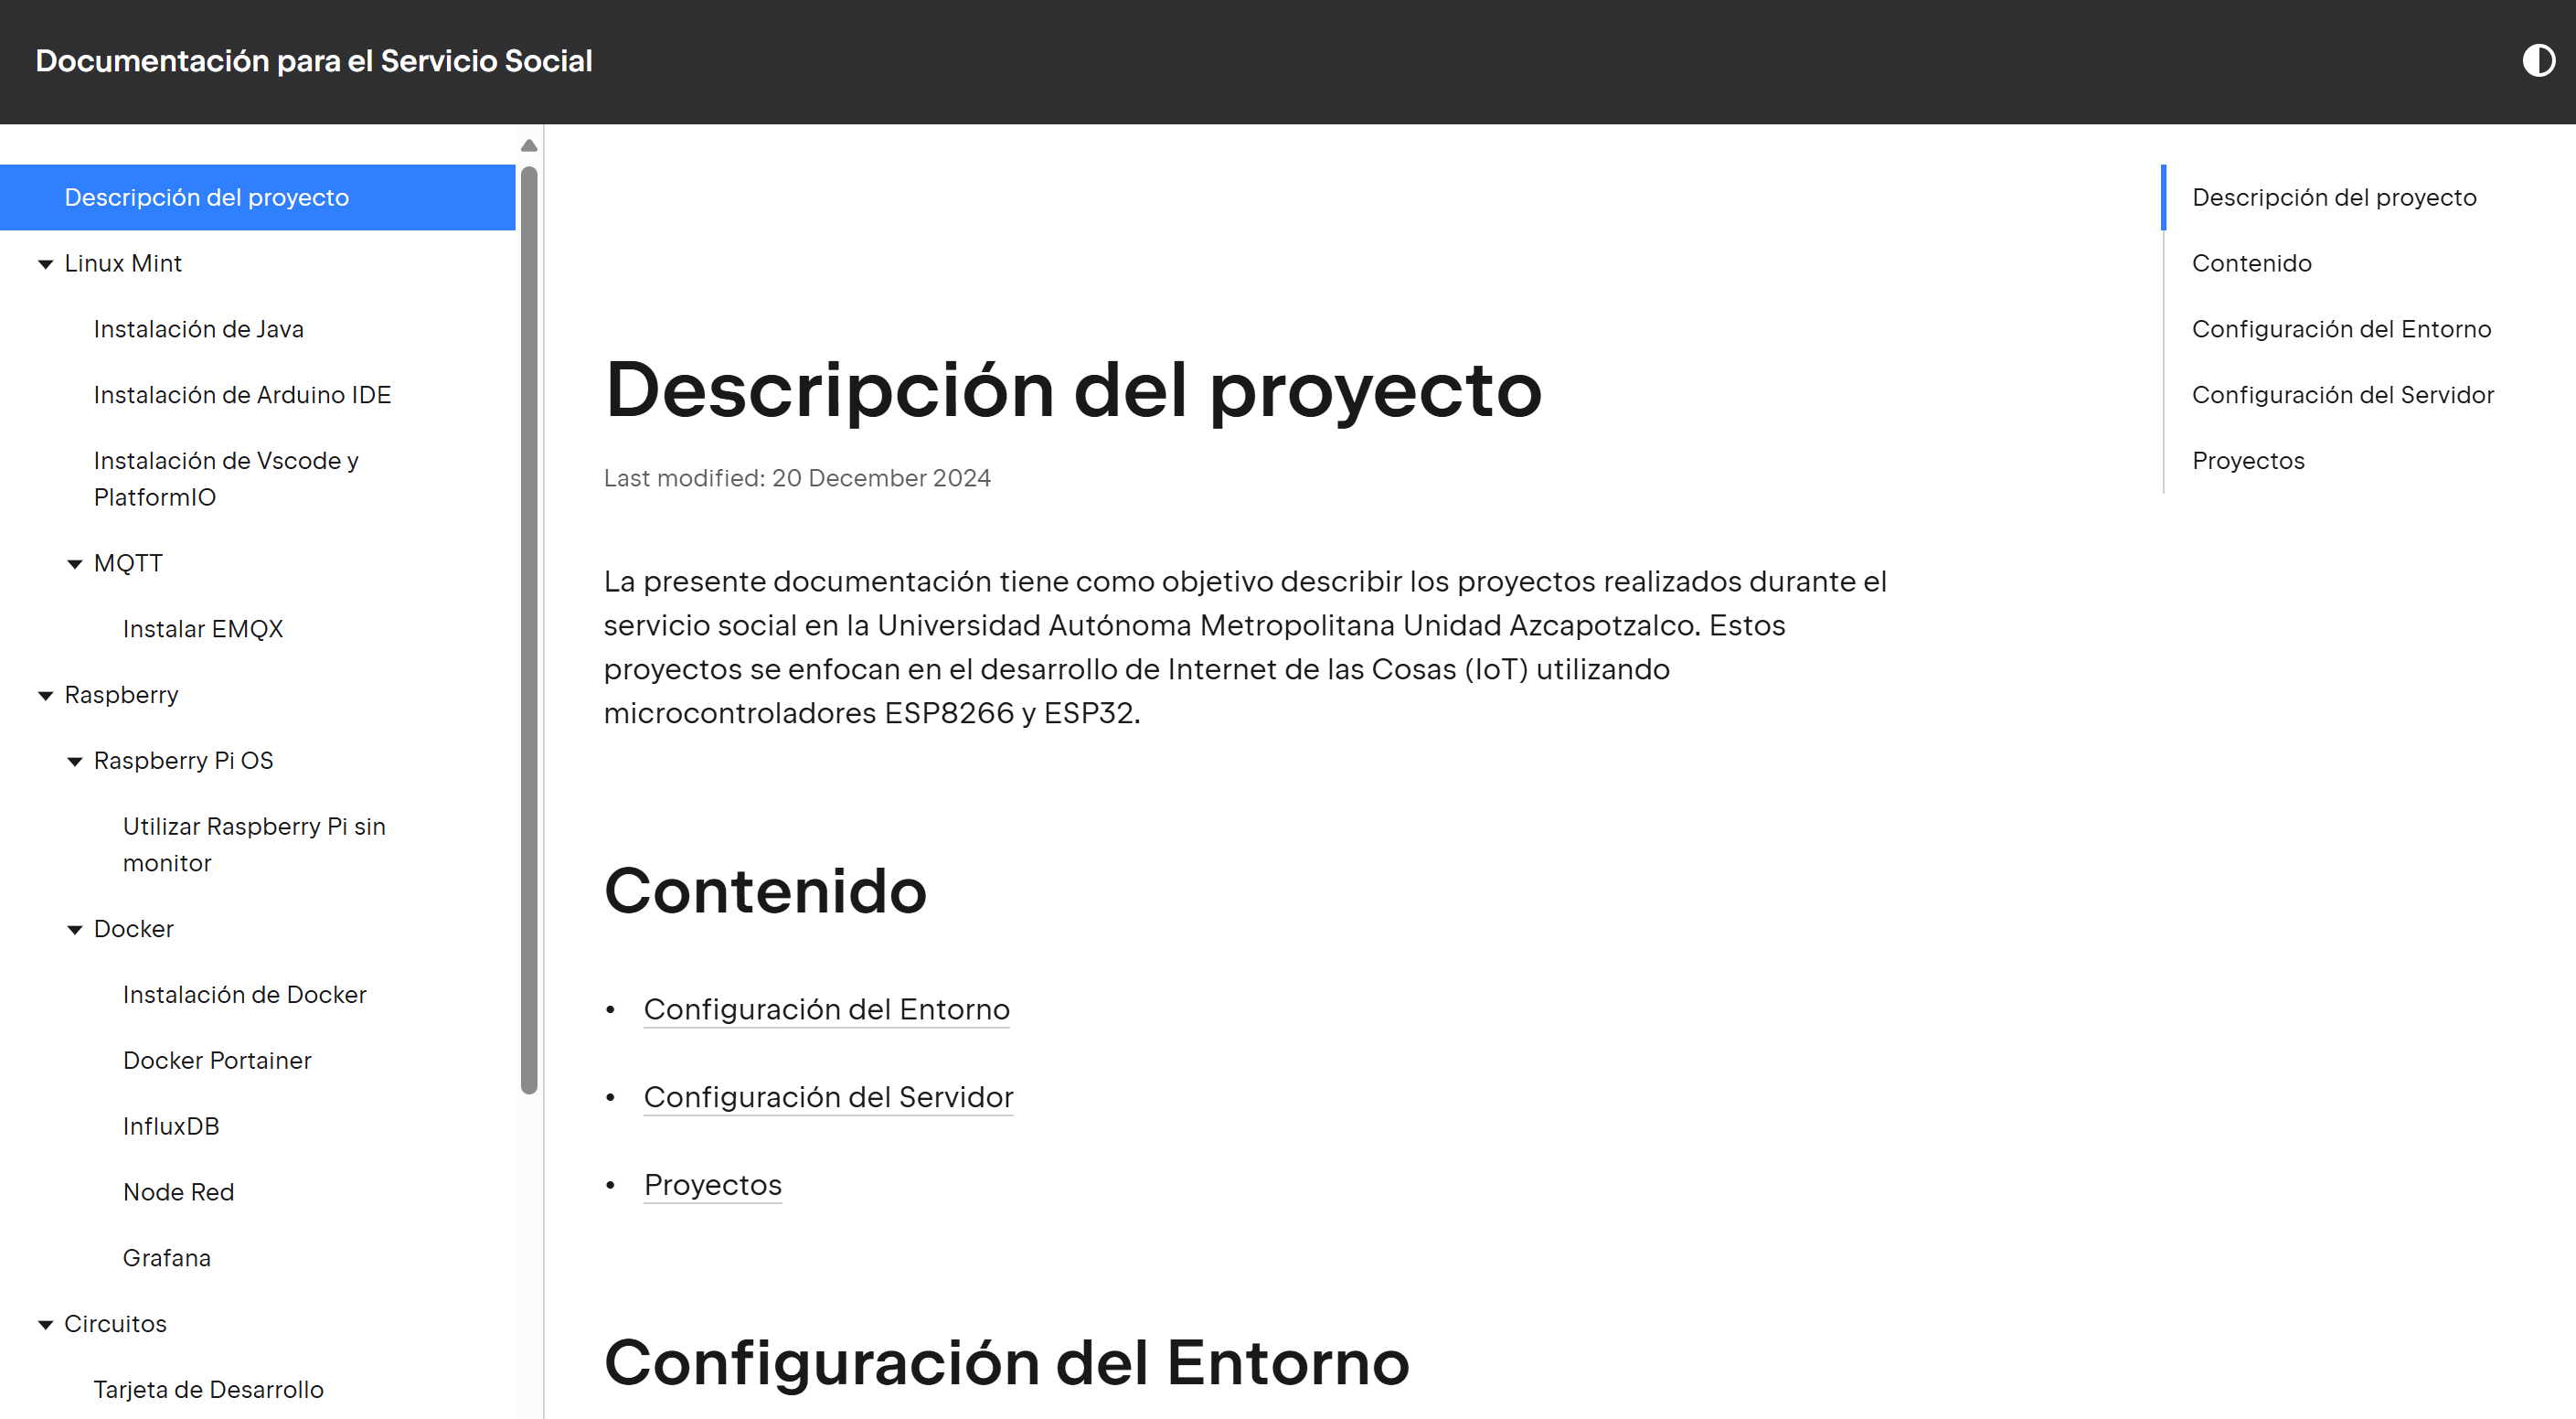
\includegraphics[width=0.8\textwidth]{img/paginaWeb.png}
    \caption{Pagina Web de la documentación del proyecto}
    \label{fig:paginaWeb}
\end{figure}

La documentación en la página web ha sido diseñada para replicar el proyecto utilizando cualquier placa de desarrollo. Para mostrar el código adaptado a la placa seleccionada, debe elegirse la placa en la parte superior de la página. En la figura~\ref{fig:placa} se muestra cómo realizar esta selección.

\begin{figure}[H]
    \centering
    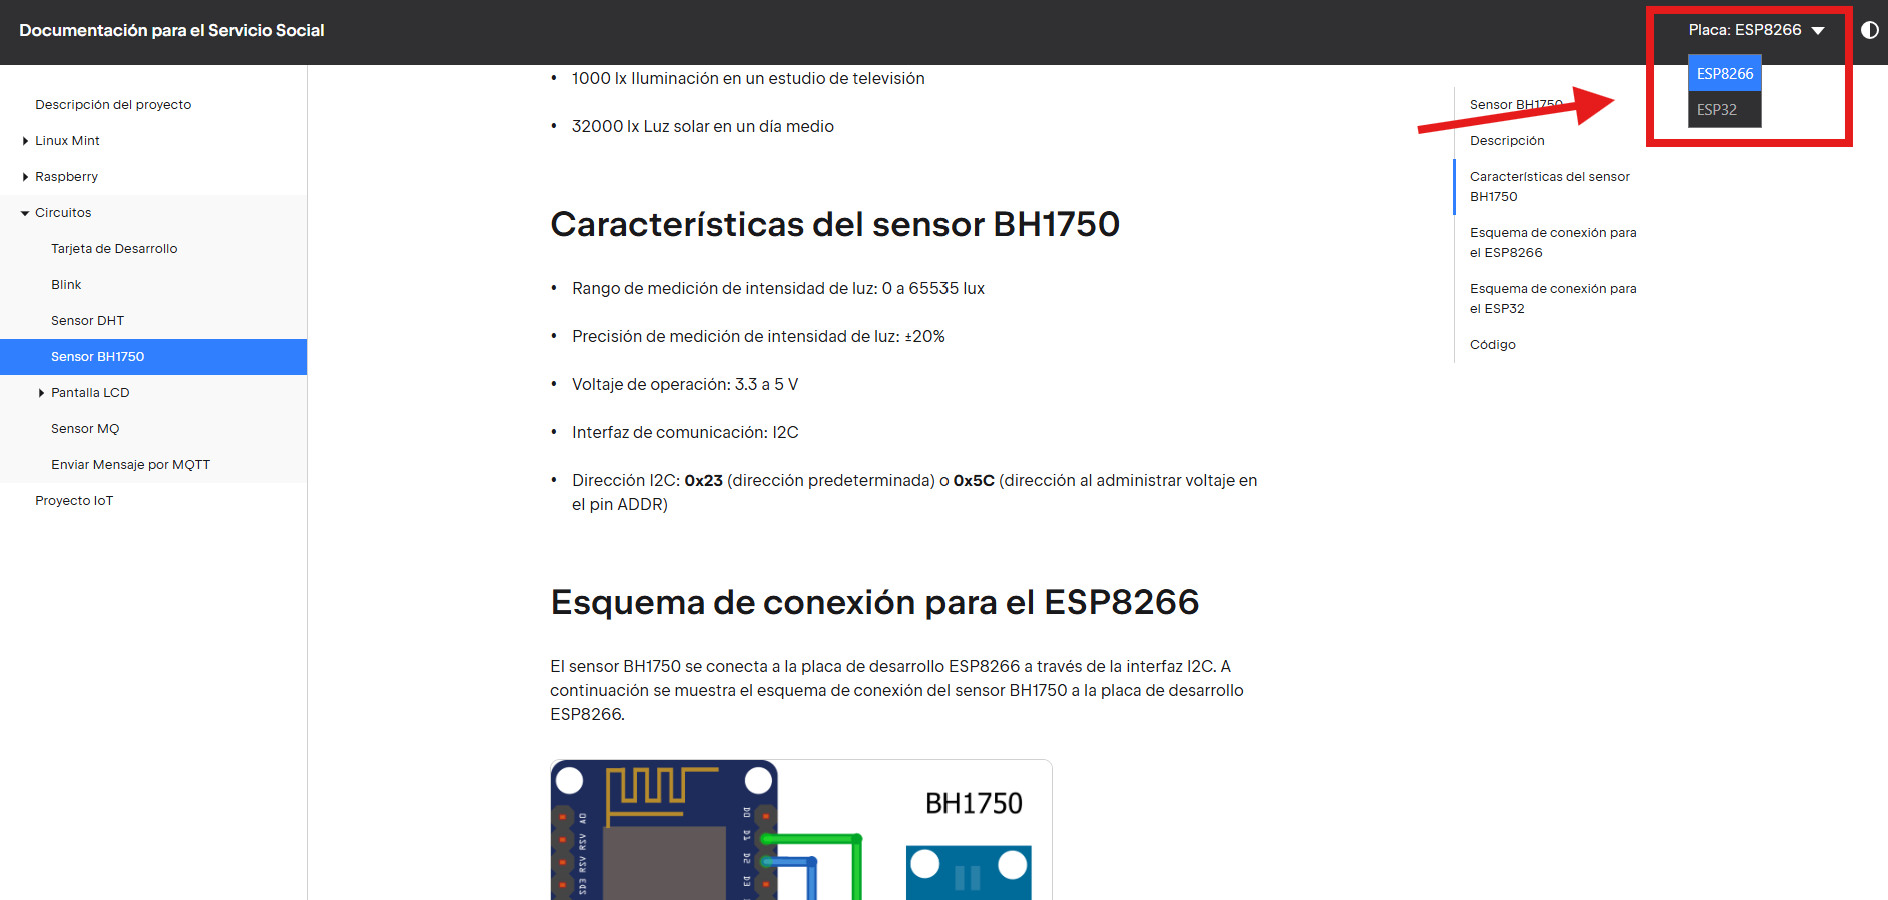
\includegraphics[width=0.8\textwidth]{img/paginaWeb_placa.png}
    \caption{Selección de la placa de desarrollo}
    \label{fig:placa}
\end{figure}

\section{Recomendaciones}

\begin{itemize}
    \item Realizar pruebas de estrés en el servidor para evaluar su capacidad de respuesta y rendimiento ante un gran número de dispositivos conectados.
    \item Implementar un sistema de copias de seguridad para garantizar la integridad de los datos almacenados en las bases de datos.
    \item Escalar el proyecto para incluir más sensores y actuadores para realizar acciones en tiempo real en función de los datos leídos.
\end{itemize}

\begin{thebibliography}{9}
    \bibitem{emqx}
    EMQ Technologies Inc. (n.d.). \url{https://www.emqx.com/en}.
    
    \bibitem{docker}
    Docker. (2024, July 8). Docker: Accelerated Container Application Development. Docker. \url{https://www.docker.com/}

    \bibitem{influxdb}
    InfluxData. (2021, December 10). InfluxDB: Open Source Time Series Database | InfluxData. \url{https://www.influxdata.com/products/influxdb/}

    \bibitem{nodered}
    Node-RED. (n.d.). Node-RED. \url{https://nodered.org/}

    \bibitem{grafana}
    Grafana Labs (n.d.). Grafana Labs | Leading observability tool for visualizations \& dashboards. \url{https://grafana.com/oss/grafana/}

    \bibitem{esp32}
    Espressif Systems. (n.d.). ESP32 - Espressif Systems. \url{https://www.espressif.com/en/products/socs/esp32}

    \bibitem{esp8266}
    Espressif Systems. (n.d.). ESP8266 - Espressif Systems. \url{https://www.espressif.com/en/products/socs/esp8266}
\end{thebibliography}
